\documentclass{ctexart}

\usepackage{pdfpages}
\usepackage{geometry}
\geometry{left=3.18cm,right=3.18cm,top=2.54cm,bottom=2.54cm}


% 设置目录显示的深度
\setcounter{tocdepth}{3}

% 设置标号深度
\setcounter{secnumdepth}{3}

% 正文区
\begin{document}

    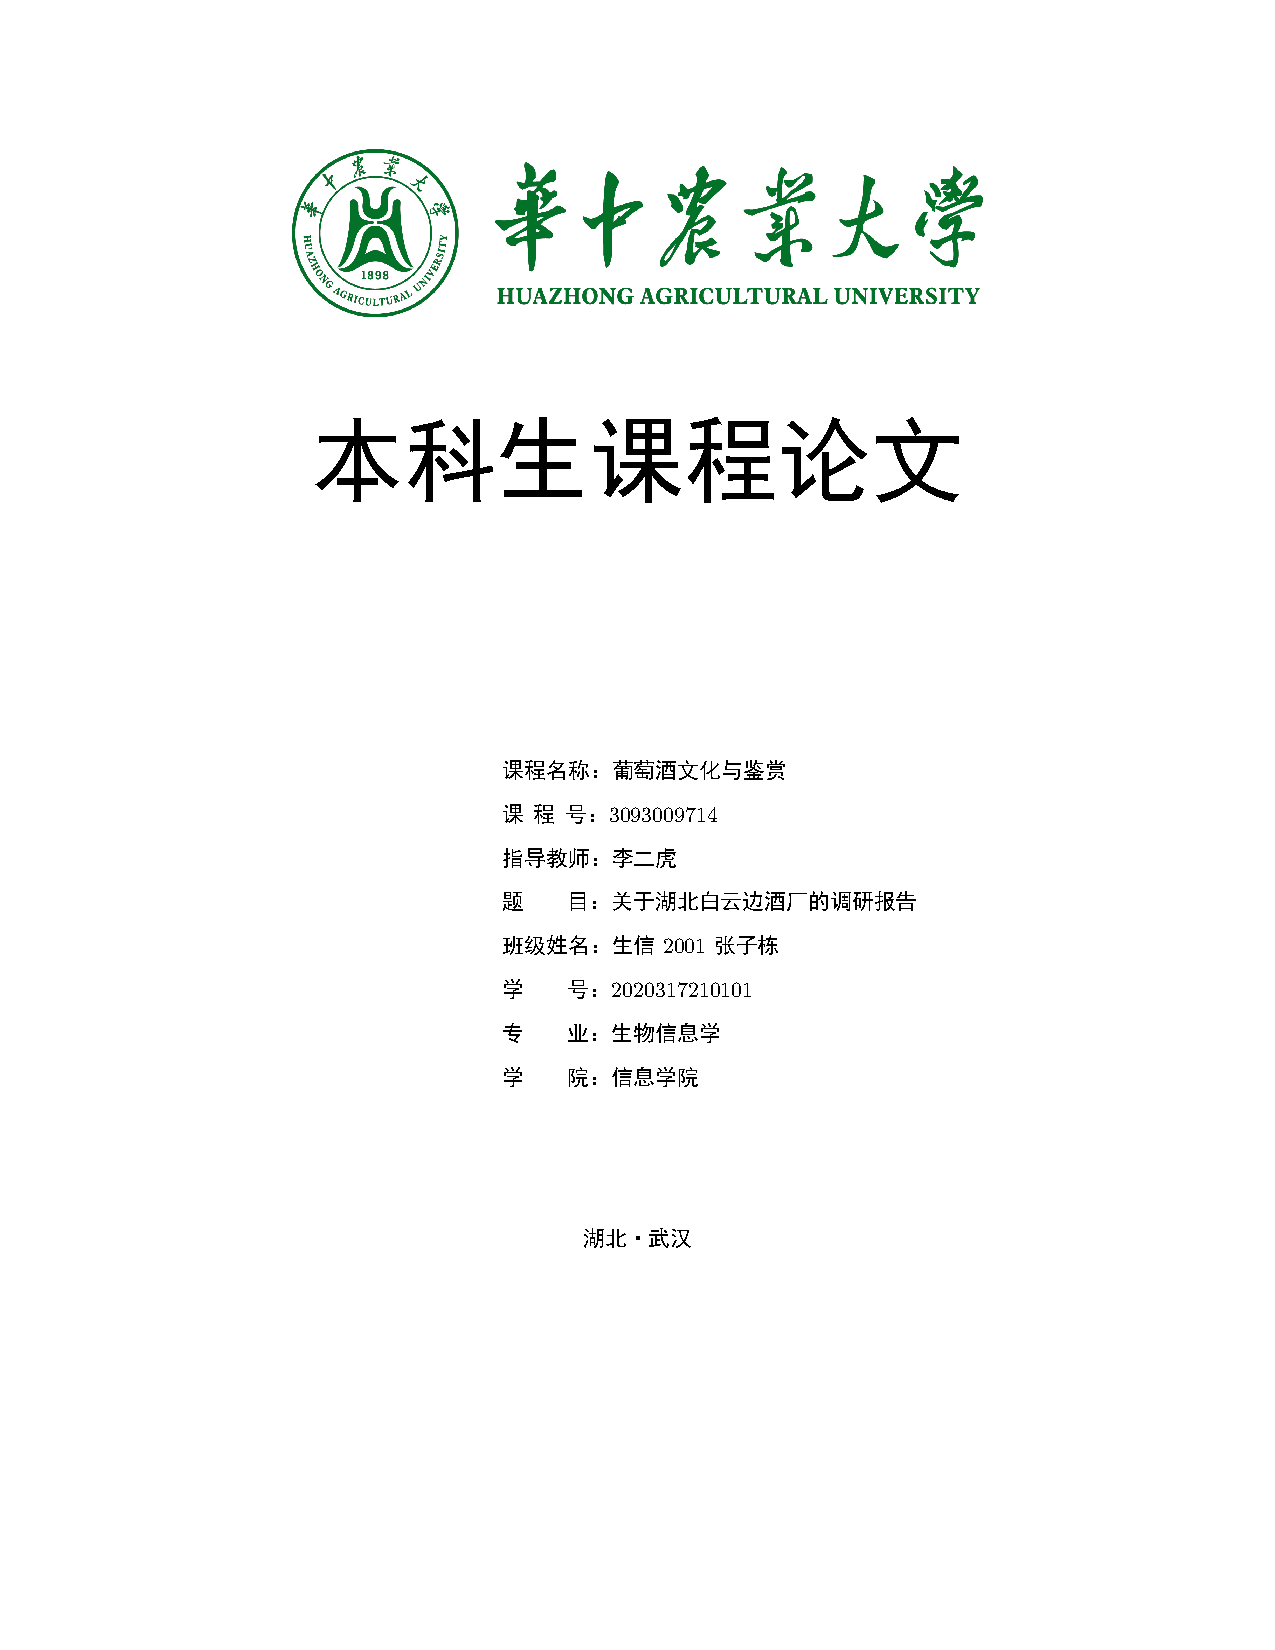
\includepdf[pages={1}]{cover.pdf}

    \clearpage

    \thispagestyle{empty}

    \begin{abstract}
        我的家乡是湖北武汉,在武汉,白云边是最常见的白酒,无论是在餐桌上还是送礼,白云边通常是武汉人的首选。白云边酒厂是一家位于湖北省松滋市的白酒生产企业,以其独创的浓酱兼香型白酒酿造技术,酿造出“中国白酒第五香”。白云边酒厂成立于2007年,注册资本30000万人民币,是湖北白云边集团的核心企业。白云边酒厂占地1300亩,总资产达80余亿元,在职员工7000余人。白云边酒厂的主要产品有1979、二十年和云酱系列等,是中国浓酱香型酒标准的起草单位之一,也是全国酿酒行业重点白酒企业。
    \end{abstract}

    \clearpage

    \tableofcontents
    
    % 目录设为页码 0(从正文起为第一页)
    

    % 目录的页脚设为空
    \thispagestyle{empty}

    \clearpage
    \quad
    \thispagestyle{empty}
    \clearpage

    \setcounter{page}{1}

    \section{白云边酒厂的历史沿革}
    白云边酒厂是湖北荆州松滋市的一家白酒品牌,以生产浓酱兼香型白酒为主。白云边酒厂的历史可以追溯到民国时期的松滋老字号“泰顺和糟坊”,其历史沿革可以概括为以下几个阶段:

    \begin{itemize}
    \item 1952年,泰顺和糟坊更名松滋县人民酒厂,从此开始了其艰辛而光荣的发展之路,以当地优质的水源和粮食为原料,开始酿造白酒。酒厂成立后不久便发展了6家分厂,员工达到100多名,年产白酒100余吨。
    \item 1979年至1989年,白云边酒连续三次获得全国白酒质量评比银质奖,成为全国知名的优质白酒品牌。
    \item 1991年,白云边酒被轻工部确定为全国浓酱兼香型白酒的典型代表,其产品风格为“芳香优雅,酱浓、协调,绵厚甜爽,圆润怡长”。
    \item 1994年,白云边酒厂改制为湖北白云边股份有限公司,开始进行市场化经营。
    \item 2005年,白云边进行了“国有股份退出、实行民有民营”的产权制度改革,成立湖北白云边集团。
    \item 2006年至2009年,白云边获得了多项国家级和行业级的荣誉和认证,如“中国白酒工业十大竞争力品牌”、“中国驰名商标”、“浓酱兼香型白酒国家标准”的起草单位等。
    \item 2007年至2010年,白云边启动了工业园项目,扩大了生产规模和产能,实现了综合产能整体翻番。
    \item 2010年至现在,白云边继续进行技术创新和市场拓展,投资建设了四川基酒基地、武汉企业总部大楼等项目。目前,白云边已经成为全省最大的优质固态白酒生产企业。
    \end{itemize} 

    从白云边的产品来看,早起的白云边酒主义生产小曲酒,1972年,酒厂借鉴名酒经验,开始试制大曲酒,“松江大曲”属于酒厂早期的大曲酒,由于与哈尔滨已注册的“松江大曲”重名,于是改名“白云边”。其后随酿造工艺的改进发展,勾调出目前广受好评的浓酱兼香型白酒。

    
    \section{白云边酒的文化}
    \subsection{白云边酒名的由来}
    公元759年,唐代大诗人李白秋游洞庭,乘流北上,夜泊湖口(今湖北松滋市境内),籍湖光月色,举杯吟诗:南湖秋水夜无烟,耐可乘流直上天,且就洞庭赊月色,将船买酒白云边。美酒绝句相得益彰,白云边酒由此得名。
    \subsection{白云边的企业文化}
    白云边以“百年品牌,幸福企业”为企业愿景,同时坚持三大价值关系:企业与社会的价值关系,体现为“以人为本、科学发展、回报社会”的企业核心价值观;企业与消费者的价值关系,体现为“敬业、协力、创新、进取”企业精神;企业与员工的价值关系,体现为独具白云边特色的“家园文化”。此外还包括“一站一报”宣传平台、职工救助基金、“送温暖”活动、“白云边杯”羽毛球赛、“白云边杯”羽毛球赛五大文化载体。

    \section{白云边酒的酿造工艺}
    白云边酒在酿造工艺上吸收了酱香型酒的精华和浓香型酒的工艺核心,把两种香型的生产工艺创造性地结合在一起,形成了白云边独特的浓酱兼香型白酒酿造技术。白云边每年九月开始投料,历经三次投料、十轮操作、九次发酵、六轮堆积,清蒸清烧和混蒸续渣相结合,长达一年的酿造周期让酒液充分吸收原料精华,最终酿成“芳香优雅,酱浓协调,绵厚甜爽,圆润怡长”的白云边酒。

    \subsection{白云边酿造中的酱香工艺}
    白云边酿造中使用到的酱香工艺主要包括高温曲和高温堆积。高温曲是指在糖化发酵过程中,将大曲的糖化温度控制在60~℃以上,这样可以使得糖化速度加快,同时也可以使得糖化产物更多地转化为有利于酒体口感的物质。高温堆积是指在发酵过程中,将发酵液的温度控制在40~℃以上,这样可以使得发酵速度加快,同时也可以使得发酵产物更多地转化为有利于酒体口感的物质。

    \subsection{白云边酿造中的浓香工艺}
    白云边酿造中使用到的浓香工艺主要包括续渣发酵和泥窖增香。续渣发酵是指在蒸馏前将上一轮的醅渣加入到新一轮的发酵液中进行发酵,这样可以使得新一轮的发酵液中含有更多的微生物和有利于口感的物质。泥窖增香是指在陈放过程中,将白云边酒放置于泥窖中进行陈放,这样可以使得白云边酒吸收泥窖中的气味和湿度,从而增加其香气和口感。

    \section{白云边酒厂的产品}

    白云边酒的产品分类主要分为:白云边酒、白云边年份酒、白云边珍品酒、白云边特制酒、白云边特曲酒等。其中,白云边酒是主打产品,包括浓香型和兼香型两种香型,年份一般为3年、5年、8年、10年等。


    \begin{itemize}
        \item 白云边年份酒是以年份命名的系列产品,包括12年、15年、20年等不同年份的产品。
        \item 白云边珍品酒是以珍品命名的系列产品,包括“金质珍品”、“银质珍品”、“铜质珍品”等不同档次的产品。
        \item 白云边特制酒是以特制命名的系列产品,包括“特制浓香型”、“特制兼香型”等不同香型的产品。
        \item 白云边特曲酒是以特曲命名的系列产品,包括“特曲浓香型”、“特曲兼香型”等不同香型的产品。
    \end{itemize}

    \section{白云边酒厂的市场}

    1998年开始,白云边以武汉市场为中心,以湖北市场为根据地,取得了湖北省第一的好成绩。在省外市场,白云边的产品结构也呈现升级的趋势。在3星、4星、5星基础上推出了次高端价位的7星陈酿,并开始将省内已打出影响力的年份陈酿系列导入省外市场,同步推高产品价位。白云边外省市场表现最为亮眼的就是河南市场。

    白云边对经销商的管理也十分精细,不同区域、不同系列、不同年份、甚至不同度数的产品都会由不同的经销商来运营。品牌方与经销商签订包销协议,在一定程度上实现了紧密的厂商协同,不仅有利于壮大经销商团队,实现对湖北主流价位带的占据。同时,也避免了经销商之间的直接竞争,有利于保持队伍和谐。

\end{document}